\documentclass[acmsmall,nonacm]{acmart}

\usepackage{booktabs}
\usepackage{amsmath}
\usepackage{amsthm}
\usepackage{bbm}
\usepackage{graphicx}
\usepackage{xcolor}
\usepackage{enumitem}
\setlist{nosep,leftmargin=*}

\newcommand{\1}{\mathbbm{1}}
\newcommand{\sigmoid}{\operatorname{logit}^{-1}}
\newcommand{\E}{\mathbb{E}}
\newcommand{\Var}{\operatorname{Var}}
\newcommand{\TODO}[1]{\textcolor{red}{\textbf{[TODO: #1]}}}
\newcommand{\DeltaCV}{\Delta_{\text{CV}}}

\newtheorem{theorem}{Theorem}
\newtheorem{proposition}{Proposition}
\newtheorem{definition}{Definition}

\settopmatter{printacmref=false}
\setcopyright{none}
\renewcommand\footnotetextcopyrightpermission[1]{}
\pagestyle{plain}

\begin{document}

%\title{The Autocorrelation Mirage: Pseudoreplication Dominates Label Leakage in Panel Forecasting}
\title{The Autocorrelation Mirage: Pseudoreplication Dominates Leakage in Rare-Event Panel Forecasting}

\author{Behnaz Moradi-Jamei}
\email{moradibx@jmu.edu}
\affiliation{\institution{James Madison University}\country{USA}}
\author{Heman Shakeri}
\email{hs@virginia.edu}
\affiliation{\institution{University of Virginia}\country{USA}}


\begin{abstract}
Rare-event forecasting from panel data faces a sample-size barrier: too few episodes for stable inference. A common solution expands episodes into daily observations, but this activates a failure mode we call \emph{episode memorization}: models learn to identify which episode an observation belongs to rather than predicting event risk. We show that standard K-Fold cross-validation---the default in libraries like Scikit-Learn---enables this failure by allowing the same episode to appear in both training and test sets. The result is dramatic: AUC inflates from 0.56 to 0.86 (+54\%) with \textit{no data leakage whatsoever}. This exceeds even explicit time-to-event leakage (+39\%). While prior work formalized leakage for i.i.d.\ data (Kaufman et al.) and block CV for spatial dependence (Roberts et al.), neither identified that \textit{pseudoreplication alone} dominates in panel-expanded forecasting. We propose the $\DeltaCV$ diagnostic: the gap between random and grouped CV estimates. In our simulation, $\DeltaCV = 0.30$---a gap this large indicates the model exploits autocorrelation structure rather than learning generalizable signal. This pathology affects conflict prediction, clinical deterioration, equipment failure, and customer churn systematically.
\end{abstract}

\keywords{pseudoreplication, cross-validation, panel data, rare events, episode memorization}
\maketitle

\section{Introduction}

Predicting rare events---coups, equipment failures, patient deterioration---from panel data confronts a sample-size barrier. With 20--50 episodes and 10--20 features, events-per-variable (EPV) ratios fall below 1.0, far short of the 10--20 required for stable inference~\cite{peduzzi1996,vansmeden2016}. A common solution expands each episode into daily rows: 20 episodes become 500+ observations, apparently resolving the problem.

We show this reformulation activates a failure mode we call \textbf{episode memorization}. When standard K-Fold cross-validation---the default in Scikit-Learn and similar libraries---assigns observations to folds, the same episode appears in both training and test sets. Because consecutive observations $X_{e,t}$ and $X_{e,t+1}$ are highly autocorrelated, the model effectively performs nearest-neighbor classification: it learns to identify the episode's identity (``this is the high-variance episode'') rather than the event risk. At test time, recognizing familiar autocorrelation patterns yields artificial accuracy. Random CV thus transforms a \textit{forecasting} problem (extrapolation to unseen episodes) into an \textit{interpolation} problem (pattern-matching within known episodes).

In our simulation, this single methodological choice---\texttt{KFold} instead of \texttt{GroupKFold}---inflates AUC from 0.56 to 0.86. This 54\% inflation occurs with strictly causal features containing \textit{no leakage whatsoever}. Remarkably, this exceeds explicit time-to-event leakage (+39\%), where features directly encode $T_e - t$. This finding reframes the rare-event forecasting literature. Kaufman et al.~\cite{kaufman2012} formalized data leakage and ``learn-predict separation,'' but focused on i.i.d.\ settings with explicit feature violations. Roberts et al.~\cite{roberts2017} established that block CV is ``nearly universally more appropriate'' for structured data, but addressed spatial dependence in ecology. Hurlbert~\cite{hurlbert1984} coined ``pseudoreplication''---finding it in 48\% of ecological studies---but addressed experimental design, not ML evaluation. We show that panel expansion creates a setting where pseudoreplication \textit{dominates} leakage: the standard tool is more dangerous than the worst feature-engineering error.

Kapoor and Narayanan~\cite{kapoor2023} documented leakage in 294+ papers across 17 fields; Neunhoeffer and Sternberg~\cite{neunhoeffer2019} showed CV misuse invalidated civil war prediction claims. We extend this by: (1)~demonstrating pseudoreplication as the dominant failure mode; (2)~formalizing episode memorization as the mechanism; (3)~proposing the $\DeltaCV$ diagnostic; and (4)~providing a corrected protocol.

\section{Theoretical Framework}\label{sec:theory}

Consider $E$ episodes indexed by $e$. Each has time $t \in \{0,\ldots,T_{\max}\}$, event time $T_e$, features $X_{e,t} \in \mathbb{R}^p$, and static attributes $\alpha_e$. For horizon $H$, the target is $Y_{e,t}(H) := \1\{t < T_e \leq t + H\}$, evaluated when at-risk ($t < T_e$).

Let $\mathcal{F}_{e,t^-} := \sigma(\{X_{e,s} : s < t\} \cup \{\alpha_e\} \cup \mathcal{E}_{<t})$ denote information strictly before $t$.

\begin{definition}[Predictable Feature]
Feature $X_{e,t}$ is \emph{predictable} if $X_{e,t} \in \mathcal{F}_{e,t^-}$---measurable with respect to information available before $t$.
\end{definition}

This extends Kaufman et al.'s~\cite{kaufman2012} learn-predict separation to filtrations. Violations need not be explicit: global statistics computed over $\{X_{e,s} : s \leq T_e\}$ implicitly depend on $T_e$.

\begin{theorem}[Leakage Guarantees Inflation]\label{thm:leakage}
If $X_{e,t} = f(T_e - t) + \epsilon_{e,t}$ with $f$ monotone and $\Var(\epsilon) = \sigma^2$, then $\lim_{\sigma^2 \to 0} \text{AUC} = 1$.
\end{theorem}

\textit{Proof sketch.} Since $Y_{e,t}(H)=1$ iff $T_e - t \in (0,H]$, monotone $f$ creates a threshold classifier that perfectly separates as noise vanishes. \qed

\section{Implicit Violations in Standard Pipelines}\label{sec:implicit}

Global normalization $\tilde{X} = (X - \mu)/\sigma$ uses statistics from all observations. When features exhibit within-episode trends toward the event, $\mu$ and $\sigma$ depend on $\{T_e\}$, creating implicit leakage. \textit{Correction:} fold-specific or rolling statistics. Mean imputation uses future observations; episode-mean imputation uses $\bar{X}_e$ which depends on $T_e$. \textit{Correction:} forward-fill only.
Centered moving averages use future values. \textit{Correction:} trailing windows only.

\begin{table}[t]
\centering
\caption{Common operations and predictability violations.}\label{tab:violations}
\vspace{-2mm}
\begin{tabular}{@{}lll@{}}
\toprule
Operation & Standard (Violates) & Corrected \\
\midrule
Normalization & Global $(\mu,\sigma)$ & Rolling/fold-specific \\
Imputation & Column/episode mean & Forward-fill only \\
Moving average & Centered window & Trailing window \\
Lag features & Include $t, t{+}1$ & Strictly $s < t$ \\
\bottomrule
\end{tabular}
\vspace{-3mm}
\end{table}

These traps require features with pre-existing trends toward the event. Strictly causal features (constructed only from past values) are immune. Real-world features often exhibit such trends---vital signs deteriorating before death, SMART errors accumulating before drive failure, conflict indicators escalating before war---making these traps practical concerns even when absent in synthetic benchmarks.

\section{Episode Memorization: The Dominant Failure}\label{sec:pseudo}

Even with leak-free features, standard K-Fold CV inflates performance through \emph{episode memorization}. This is Hurlbert's~\cite{hurlbert1984} pseudoreplication translated to ML: ``replicates are not statistically independent.'' Within-episode observations share: (1)~latent episode effects $\alpha_e$; (2)~autocorrelated features with $\text{Corr}(X_{e,t}, X_{e,t+1}) \gg 0$; (3)~labels determined by the same $T_e$. When random CV places observations from episode $e$ in both training and test sets, the model learns episode-specific patterns---the ``texture'' of each episode's autocorrelation structure. At test time, it performs \textit{identity inference}: recognizing which episode an observation belongs to, then recalling the associated outcome. This transforms forecasting (extrapolation) into interpolation (pattern-matching). Under intraclass correlation $\rho$ with $m$ observations per episode:
$n_{\text{eff}} = \frac{n}{1 + (m-1)\rho}$.


For $n=600$, $m=20$, $\rho=0.5$: $n_{\text{eff}} = 55$---a 10$\times$ reduction. But the inflation from episode memorization is \textit{not} merely a sample-size effect: even with $n_{\text{eff}} < 20$, random CV achieves AUC $> 0.8$ (Figure~\ref{fig:simulation}D).

\begin{proposition}
Under within-episode dependence ($\rho > 0$): $\E[\widehat{\text{AUC}}_{\text{random}}] > \E[\widehat{\text{AUC}}_{\text{grouped}}]$, with gap increasing in $\rho$ and model capacity.
\end{proposition}

\section{Empirical Validation}\label{sec:empirical}
We generate $E=30$ episodes with: episode effect $\alpha_e \sim \mathcal{N}(0,0.5)$; AR(1) latent process $Z_{e,t} = 0.7 Z_{e,t-1} + \epsilon_t$; hazard $h_{e,t} = \sigmoid(-3 + \alpha_e + 0.15 Z_{e,t})$; features from $Z_{e,<t}$ only (strictly causal); label $Y_{e,t} = \1\{t < T_e \leq t+14\}$.
The intercept $-3$ yields an approximate $5\%$ base event rate
($\operatorname{logit}^{-1}(-3)\approx 0.047$), matching empirical rare-event
frequencies. Features are constructed only from $Z_{e,<t}$ (strictly causal);
the label is $Y_{e,t}=\mathbbm{1}\{\, t < T_e \le t+14 \,\}.$
We evaluate four conditions across 100 replicates.

\begin{table}[t]
\centering
\caption{Simulation results (100 replicates). Pseudoreplication dominates leakage.}\label{tab:sim}
\vspace{-2mm}
\begin{tabular}{@{}lccc@{}}
\toprule
Condition & AUC & Brier & Inflation \\
\midrule
Leak-Free + Grouped CV & 0.56 $\pm$ 0.07 & 0.29 $\pm$ 0.05 & baseline \\
Leak-Free + Random CV & \textbf{0.86 $\pm$ 0.04} & 0.15 $\pm$ 0.02 & \textbf{+54\%} \\
Norm.\ Leak + Grouped & 0.56 $\pm$ 0.07 & 0.29 $\pm$ 0.05 & +0\%$^\dagger$ \\
Explicit Leak + Grouped & 0.77 $\pm$ 0.04 & 0.16 $\pm$ 0.03 & +39\% \\
\bottomrule
\multicolumn{4}{l}{\footnotesize $^\dagger$See text for interpretation.}
\end{tabular}
\vspace{-5mm}
\end{table}

\begin{figure}[t]
\centering
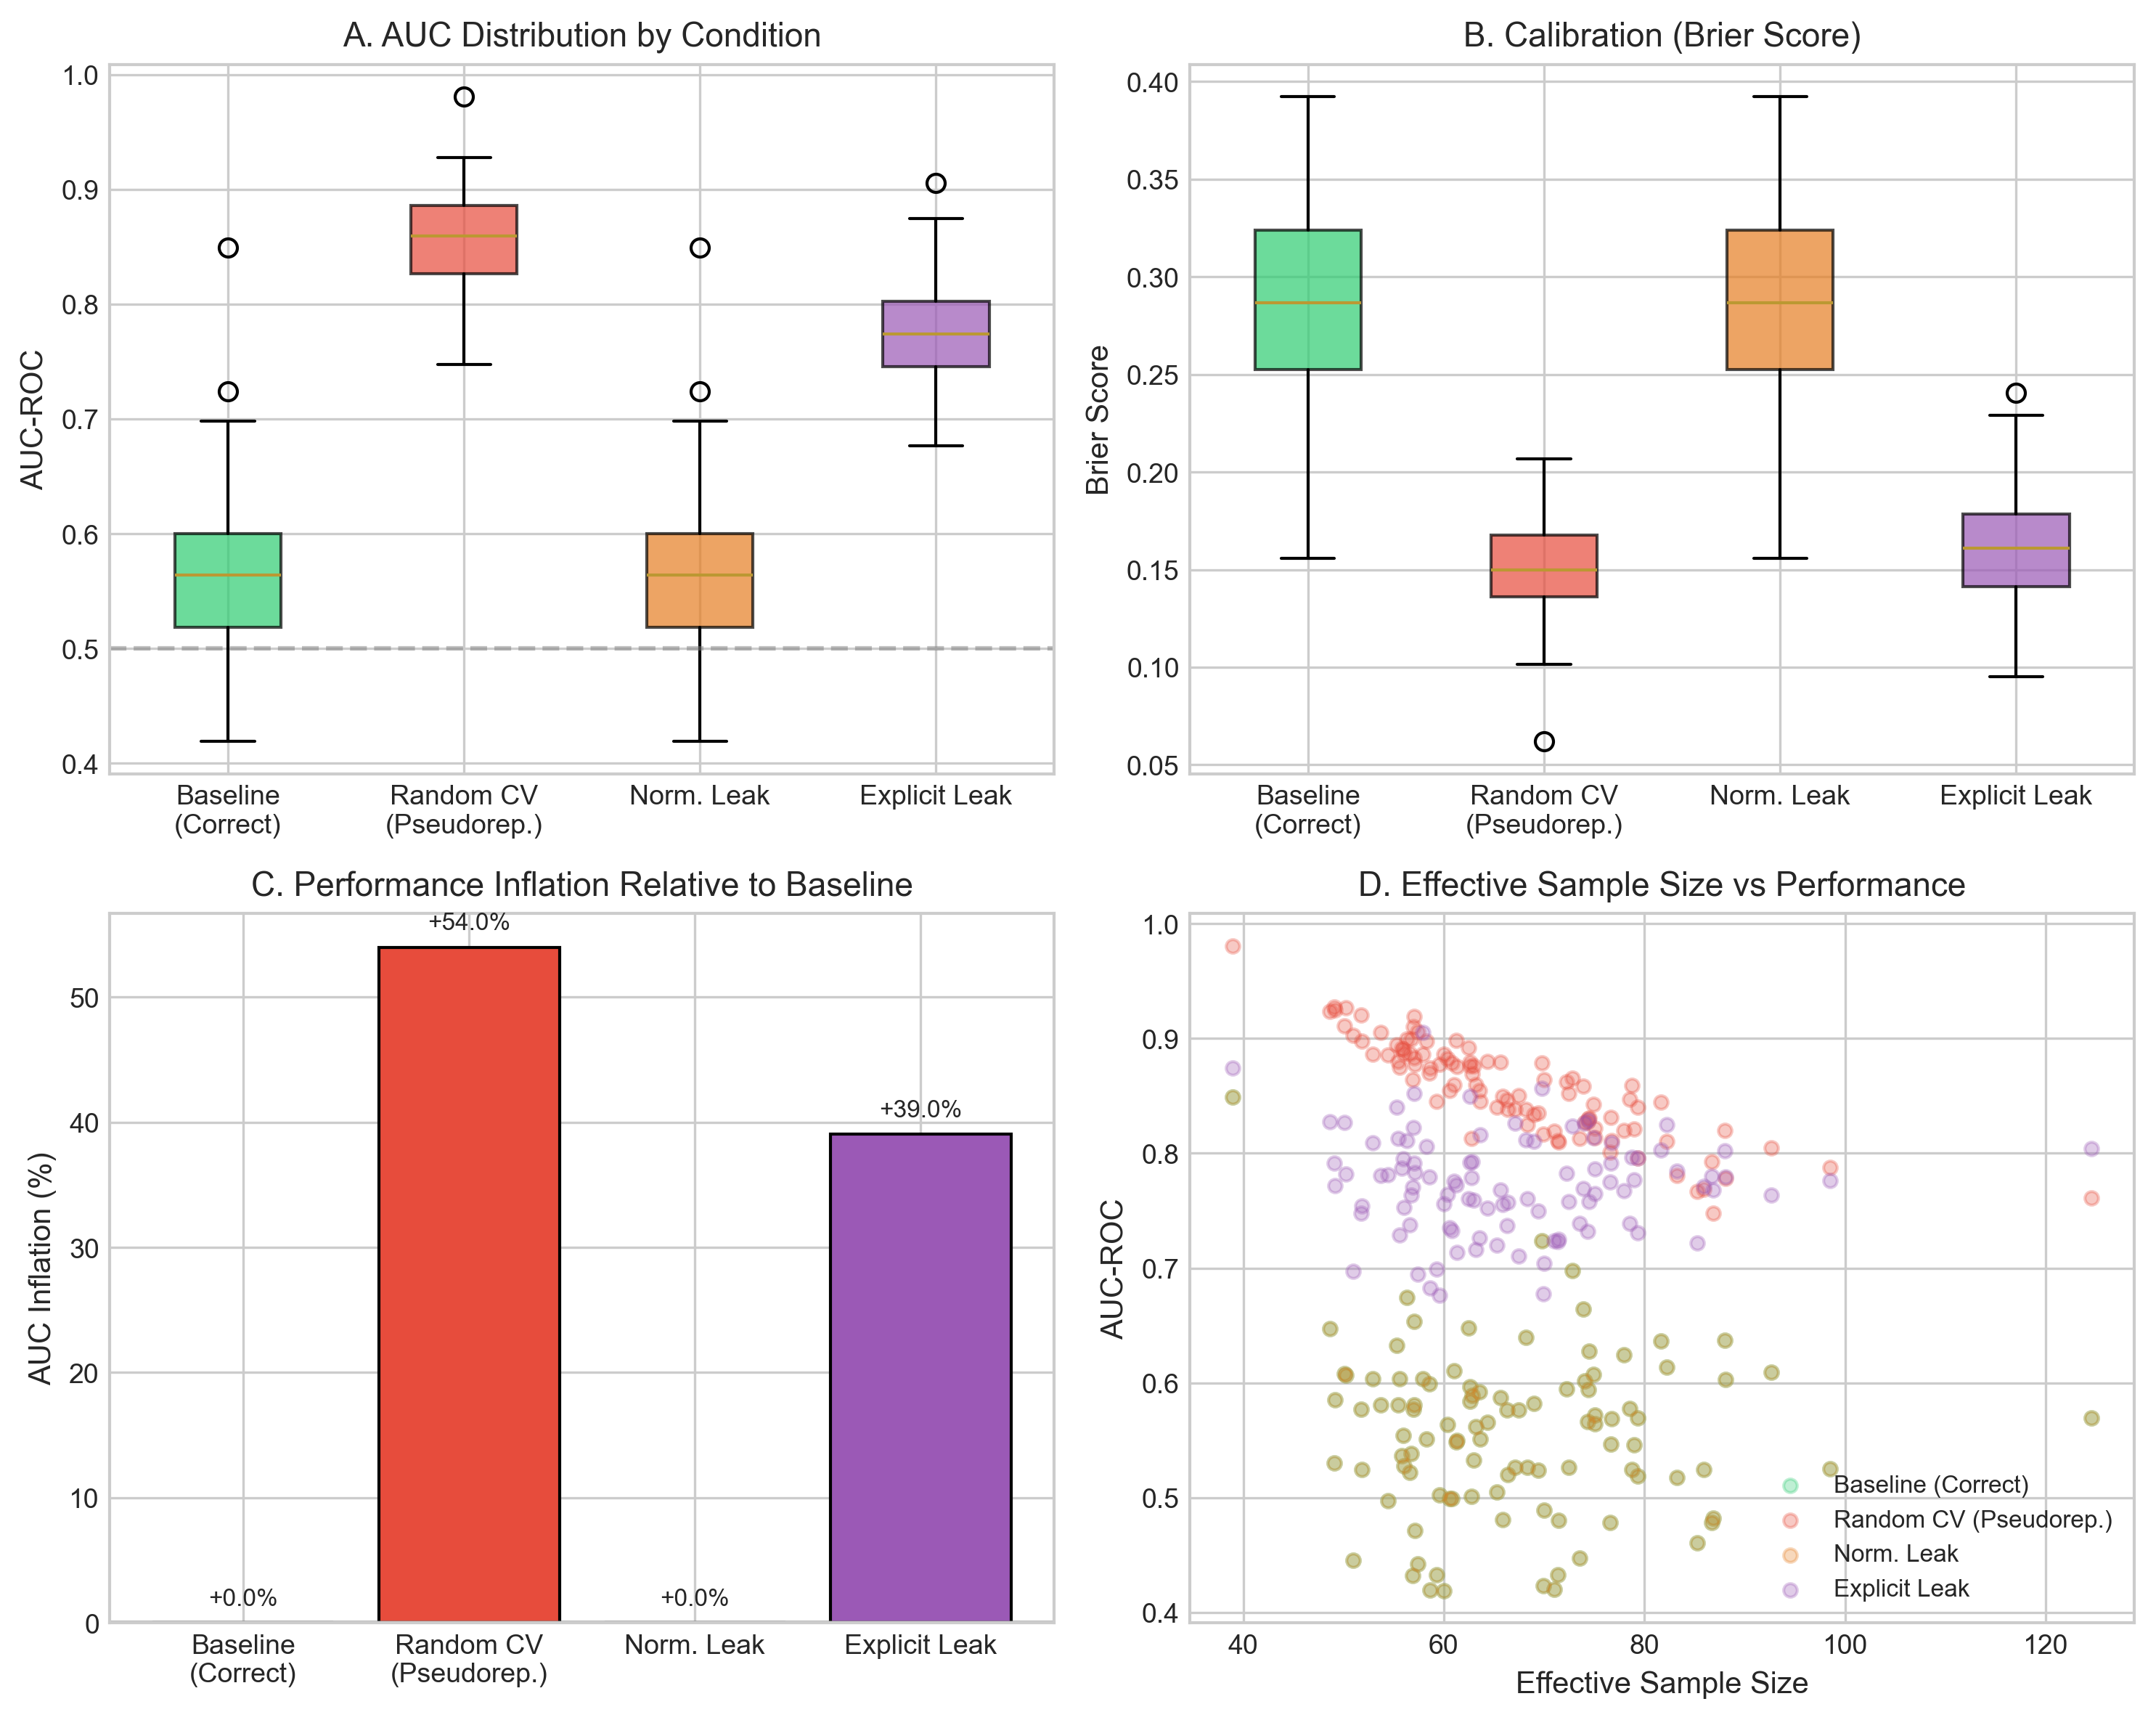
\includegraphics[width=0.7\columnwidth]{figure1_simulation_results.png}
\caption{Simulation results (100 replicates). \emph{(A)}~AUC distributions: random CV inflates performance dramatically. \emph{(B)}~Brier scores confirm improved calibration under random CV is spurious. \emph{(C)}~Pseudoreplication (+54\%) exceeds explicit leakage (+39\%)---the standard tool is more dangerous than the worst feature error. \emph{(D)}~Under random CV (red), performance completely decouples from effective sample size: the model achieves AUC $> 0.8$ even when $n_{\text{eff}} < 50$, indicating exploitation of autocorrelation artifact rather than learned signal.}
\label{fig:simulation}
\vspace{-6mm}
\end{figure}

Table~\ref{tab:sim} and Figure~\ref{fig:simulation} reveal the central finding: pseudoreplication alone inflates AUC more than explicit leakage. Random CV yields AUC=0.86 from features with no leakage---a 54\% inflation over grouped CV (AUC=0.56). The $\DeltaCV$ gap is 0.30. Explicit $T_e - t$ leakage inflates by only 39\%.  Global normalization shows +0\% inflation because our synthetic features are stationary AR(1) processes with no pre-event trends. This is a \textit{conservative} design choice, not a refutation of the normalization trap. In real-world domains with pre-event trends (deteriorating vitals, accumulating errors), the normalization trap activates. The critical finding is that pseudoreplication inflates AUC to 0.86 \textit{even in this trend-free setting}---autocorrelation alone is sufficient to destroy validity.

Figure~\ref{fig:simulation}D demonstrates that under random CV, performance completely decouples from effective sample size. The model achieves high AUC regardless of $n_{\text{eff}}$, indicating it exploits episode texture rather than learning generalizable signal.

\section{The $\DeltaCV$ Diagnostic}\label{sec:protocol}

We propose a simple diagnostic for episode memorization:

\begin{definition}[$\DeltaCV$ Diagnostic]
$\DeltaCV := \widehat{\text{AUC}}_{\text{random}} - \widehat{\text{AUC}}_{\text{grouped}}$. A gap $\DeltaCV > 0.05$ indicates the model relies on episode memorization rather than generalizable signal.
\end{definition}

In our simulation, $\DeltaCV = 0.30$. This metric requires no additional data collection---only re-running evaluation with \texttt{GroupKFold} instead of \texttt{KFold}.

\textbf{Corrected Protocol:} (1)~\textit{Preprocessing:} Fit transformations on training fold only; forward-fill imputation; trailing windows. (2)~\textit{Evaluation:} Use \texttt{GroupKFold} with \texttt{groups=episode\_id}; never split episodes across folds. (3)~\textit{Reporting:} Report $\DeltaCV$ and $n_{\text{eff}}$ alongside AUC.

\textbf{Red flags:} AUC $> 0.85$ with $E < 50$ episodes; $\DeltaCV > 0.10$; Brier $< 0.10$ on imbalanced data.

\section{Discussion}
Leakage requires specific conditions: explicit $T_e - t$ features, or trending features combined with global normalization. Pseudoreplication requires only default \texttt{KFold}---a single line of code that every practitioner uses. This asymmetry explains why pseudoreplication is the greater threat: it is invisible, ubiquitous, and activated by default.

 We unify Kaufman et al.~\cite{kaufman2012} (leakage formalization), Roberts et al.~\cite{roberts2017} (block CV), and Hurlbert~\cite{hurlbert1984} (pseudoreplication). The contribution is demonstrating that pseudoreplication \textit{dominates} in panel-expanded forecasting and providing the $\DeltaCV$ diagnostic. The pathology applies wherever rare events are expanded into panels: conflict forecasting~\cite{muchlinski2016,hegre2019}, clinical deterioration, predictive maintenance, customer churn. Our DGP uses stationary features; real-world trending features would activate the normalization trap, potentially compounding inflation beyond 54\%. We focus on gradient boosting; sequence models may have additional vulnerabilities through attention-based episode memorization.

Panel expansion creates value only if evaluation respects episode boundaries. Standard K-Fold CV---the default in Scikit-Learn---violates this, enabling episode memorization that inflates AUC by 54\%. This exceeds explicit time-to-event leakage (+39\%), making the standard tool more dangerous than the worst feature-engineering error. The $\DeltaCV$ diagnostic (random minus grouped CV) provides a simple check: our simulation shows $\DeltaCV = 0.30$. We call for retrospective audits of published rare-event forecasting claims and recommend that reviewers require grouped CV, $\DeltaCV$ reporting, and $n_{\text{eff}}$ disclosure.

\bibliographystyle{ACM-Reference-Format}
\bibliography{references}

\end{document}